\section{Spatial Extent}
\label{sec:Spatial}
%%%%%%%%%%%%%%%%%%%%%%%%%%%%%%%%%%%%%%%%%%%%%%%%%%%%%%%%
\begin{figure}[h!]
\begin{center}
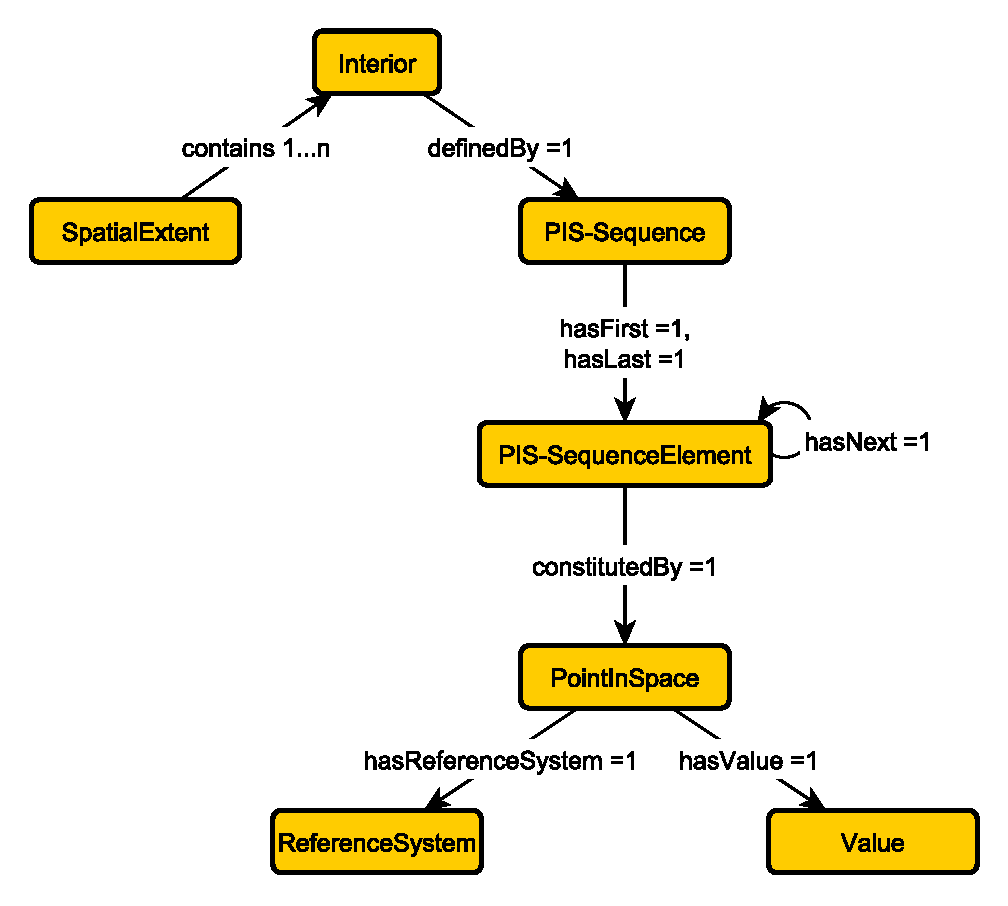
\includegraphics[width=.8\textwidth]{figures/spatial}
\end{center}
\caption{Schema Diagram for Spatial Extent. The visual notation is explained in Chapter \ref{chap:prelims}.}
\label{fig:Spatial}
\end{figure}
\subsection{Summary}
\label{sum:Spatial}
%%%%%%%%%%%%%%%%%%%%%%%%%%%%
The \textsf{SpatialExtent} pattern is characterized by a set of \textsf{Interiors}, which are in turn characterized by a \textsf{PointInSpace-Sequence}. A \textsf{PointInSpace-Sequence} consists of \textsf{PointInSpace-SequenceElements}, which are constituted by \textsf{PointInSpace}. A \textsf{PointInSpace} is described by a value and a reference system. \textsf{PIS-Sequence} is a specialization of the \textsf{Sequence} Pattern (Section \ref{sec:Sequence}). We also further choose to use the Explicit Typing Pattern for \textsf{PointInSpace} and \textsf{ReferenceSystem}.

%%%%%%%%%%%%%%%%%%%%%%%%%%%%%%%%%%%%%%%%%%%%%%%%%%%%%%%%
\subsection{Axiomatization}
\label{axs:Spatial}
%%%%%%%%%%%%%%%%%%%%%%%%%%%%
\begin{align}
\textsf{SpatialExtent} &\sqsubseteq \mathord{=}n \textsf{contains.Interior} \\
\textsf{Interior} &\sqsubseteq \mathord{=}1 \textsf{isDefinedBy.PIS-Sequence} \\
\textsf{PIS-Sequence} &\sqsubseteq \mathord{=}1 \textsf{hasFirst.PIS-SequenceElement} \\
\textsf{PIS-Sequence} &\sqsubseteq \mathord{=}1 \textsf{hasLast.PIS-SequenceElement} \\
\textsf{PIS-SequenceElement} &\sqsubseteq \mathord{=}1 \textsf{hasNext.PIS-SequenceElement} \\
\textsf{PIS-SequenceElement} &\sqsubseteq \mathord{=}1 \textsf{constitutedBy.PointInSpace} \\
\textsf{PointInSpace} &\sqsubseteq \mathord{=}1 \textsf{hasReferenceSystem.ReferenceSystem} \\
\textsf{PointInSpace} &\sqsubseteq \mathord{=}1 \textsf{hasValue.Value}
\end{align}

%%%%%%%%%%%%%%%%%%%%%%%%%%%%%%%%%%%%%%%%%%%%%%%%%%%%%%%%
\subsection{Explanations}
\label{exp:Spatial}
%%%%%%%%%%%%%%%%%%%%%%%%%%%%
\begin{enumerate}
\item Numerical Restriction: a \textsf{SpatialExtent} \textsf{contains} exactly $n$ \textsf{Interiors}. See the following section.
\item Numerical Restriction: a \textsf{Interior} \textsf{isDefinedBy} exactly 1 \textsf{PIS-Sequence}.
\item Numerical Restriction: a \textsf{PIS-Sequence} has exactly 1 first \textsf{PIS-SequenceElement}.
\item Numerical Restriction: a \textsf{PIS-Sequence} has exactly 1 last \textsf{PIS-SequenceElement}.
\item Numerical Restriction: a \textsf{PIS-SequenceElement} has exactly 1 next \textsf{PIS-SequenceElement}.
\item Numerical Restriction: a \textsf{PIS-SequenceElement} \textsf{isConstitutedBy} exactly 1 \textsf{PointInSpace}.
\item Numerical Restriction: a \textsf{PointInSpace} has exactly 1 \textsf{ReferenceSystem}.
\item Numerical Restriction: a \textsf{PointInSpace} has exactly 1 \textsf{Value}. 
\end{enumerate}

%%%%%%%%%%%%%%%%%%%%%%%%%%%%%%%%%%%%%%%%%%%%%%%%%%%%%%%%
\subsection{Remarks}
\label{rem:Spatial}
%%%%%%%%%%%%%%%%%%%%%%%%%%%%
We would also like the pattern to be able to express that a \textsf{SpatialExtent} consists of exactly some \textsf{Interiors} and no others. This is done by equipping the pattern with an axiom that must be tailored to the use-case and two rules for generating a set of assertions.

\begin{equation}
\textsf{SpatialExtent} \sqsubseteq \mathord{=}n\textsf{contains.Interior}
\end{equation}
where $n$ is the number of expected \textsf{Interiors}. Next,
$$\textit{contains}(\textsf{spatialExtent, interior}_k) \text{ for } k=1,...,n$$
and
$$\textsf{interior}_i \not = \textsf{interior}_j \text{ for } i \not = j$$
This allows us to express a \textsf{SpatialExtent} as a set of \textsf{Interiors}.
%%%%%%%%%%%%%%%%%%%%%%%%%%%%%%%%%%%%%%%%%%%%%%%%%%%%%%%%
\subsection{Competency Question}
\label{cqs:Spatial}
%%%%%%%%%%%%%%%%%%%%%%%%%%%%
\begin{enumerate}[CQ1.]
\item Where was the Battle of Manassas?
\item What path did the moose take to Canada?
\item Where is the largest prairie in the United States?
\end{enumerate}

\newpage
%%%%%%%%%%%%%%%%%%%%%%%%%%%%%%%%%%%%%%%%%%%%%%%%%%%%%%%%
% End Section
%%%%%%%%%%%%%%%%%%%%%%%%%%%%%%%%%%%%%%%%%%%%%%%%%%%%%%%%
%%%%%%%%%%%%%%%%%%%%%%%%%%%%%%%%%%%%%%%%%%%%%%%%%%%%%%%%